\documentclass[]{article}
\newcommand{\FileDepth}{../..}
\usepackage[a4paper, total={15cm,23cm}]{geometry}
\usepackage[T1]{fontenc}
\usepackage{textcomp}%Not strictly necessary, but gives \textmu command for "micro."
\usepackage{fancyhdr}
\usepackage{amsmath}
\usepackage{amssymb}
\usepackage{graphicx}
\usepackage{xcolor}
\usepackage{tikz}
\usetikzlibrary{calc}
\usepackage{cancel}%This is special for Activities 4 and 5.
%opening
\newcommand{\SecType}{X}
\newcommand{\Week}{X}
\title{Suspended Loudspeaker}
\author{Benjamin Bauml}
\date{Spring 2024}
\pagestyle{fancy}
\rhead{PH 221}
\chead{Spring 2024}
\lhead{Week \Week}

% For Assignment, leave Purpose as 1. For Worksheet, set to 2. For Student Solution, set to 3. For Teacher Solution, set to 4.
% If you want keep the pieces from being called manually, set DefOnly to 0.
\newcommand{\Purpose}{4}
\newcommand{\DefOnly}{1}

% Version 2024-04-27
% Changes
% 2024-02-21 Added xstring package to enable smooth implementation of new \ModePage command.
% 2024-04-27 Set up to split activities and formatting aspects into separate files. Removed dependence on xcomment. Added an automatic counter to number the activities in a problem set.
\usepackage{tcolorbox}
\usepackage{xstring}
% You will want the following four lines in your document (the last two uncommented):
% For Assignment, leave Purpose as 1. For Worksheet, set to 2. For Student Solution, set to 3. For Teacher Solution, set to 4.
% If you want keep the pieces from being called manually, set DefOnly to 0.
%\newcommand{\Purpose}{4}
%\newcommand{\DefOnly}{1}
\newcommand{\Exclusion}{0}
\newcommand{\PageTurn}{0}
\newcommand{\GrayProb}{0}
\newcommand{\Tipsy}{0}

% Assignment
\if\Purpose1
\renewcommand{\Exclusion}{1}
\fi
% Worksheet
\if\Purpose2
\renewcommand{\Exclusion}{1}
\renewcommand{\PageTurn}{1}
\fi
% Student Solution
\if\Purpose3
\renewcommand{\PageTurn}{1}
\renewcommand{\GrayProb}{1}
\fi
% Teaching Copy
\if\Purpose4
\renewcommand{\PageTurn}{1}
\renewcommand{\GrayProb}{1}
\renewcommand{\Tipsy}{1}
\fi

\def \NewQ {0}
\def \PForce {0}
\newcommand{\MaybePage}[1]{
	\def \PForce {#1}
	\if\PForce1
	\newpage
	\else
	\if\NewQ0
	\gdef \NewQ {\PageTurn}
	\else
	\newpage
	\fi
	\fi
}

\newcommand{\ModePage}[1]{
	\IfSubStr{#1}{\Purpose}{\newpage}{}
}

\newcounter{ActNumber}
\setcounter{ActNumber}{0}

\newcommand{\Problem}[4][0]{%The first argument is optional, and if it is set to 1, the \newpage will be forced. The second argument is the name of the activity, the third is the command the activity is stored as, and the fourth is the actual problem statement.
\newcommand{#3}{
\MaybePage{#1}
\addtocounter{ActNumber}{1}
\section*{\SecType\Week-\theActNumber: #2}
\if\GrayProb1
\begin{tcolorbox}[colback=lightgray,colframe=lightgray,sharp corners,boxsep=1pt,left=0pt,right=0pt,top=0pt,bottom=0pt,after skip=2pt]
\else
\begin{tcolorbox}[colback=white,colframe=white,sharp corners,boxsep=1pt,left=0pt,right=0pt,top=0pt,bottom=0pt,after skip=2pt]
\fi
#4
\end{tcolorbox}\noindent
}
\if\DefOnly0
\else
#3
\fi
}
	
\newcommand{\ProblemSub}[3][0]{%The first argument is optional, and if a string of numbers is entered into it, it will force a \newpage in any \Purpose that shows up in the string. For example, "13" would lead to the newpage being forced in modes 1 and 3. The second is the command the activity is stored as, and the third is the actual problem statement.
\newcommand{#2}{
\ModePage{#1}
\if\GrayProb1
\begin{tcolorbox}[colback=lightgray,colframe=lightgray,sharp corners,boxsep=1pt,left=0pt,right=0pt,top=0pt,bottom=0pt,after skip=2pt]
\else
\begin{tcolorbox}[colback=white,colframe=white,sharp corners,boxsep=1pt,left=0pt,right=0pt,top=0pt,bottom=0pt,after skip=2pt]
\fi
#3
\end{tcolorbox}\noindent
}
\if\DefOnly0
\else
#2
\fi
}
		
\newcommand{\Solution}[2]{%The first argument is the command the solution is stored as, and the second is the actual solution.
\newcommand{#1}{
\if\Exclusion0
#2
\fi
}
\if\DefOnly0
\else
#1
\fi
}
		
\newcommand{\ProblemFig}[2]{%The first argument is the command the figure is stored as, and the second is the actual figure.
\newcommand{#1}{
\begin{figure}[h]
#2
\end{figure}
}
\if\DefOnly0
\else
#1
\fi
}
		
\newcommand{\TeachingTips}[1]{
\if\Tipsy1
\begin{tcolorbox}[colback=lightgray,colframe=black]
#1
\end{tcolorbox}
\fi
}

\newcommand{\FBDaxes}[3]{
	\begin{scope}[shift={(#1)},rotate=#2]
		% x-axis
		\draw[thick,->] (-2,0) -- (2,0);
		\node[anchor=west] at (2,0) {$x$};
		% y-axis
		\draw[thick,->] (0,-2) -- (0,2);
		\node[anchor=west] at (0,2) {$y$};
		\coordinate (#3) at (0,0);
	\end{scope}
}
\newcommand{\FBDvectorMA}[4]{
	\begin{scope}[shift={(#1)}]
		\coordinate (#4tip) at ({#2*cos(#3)},{#2*sin(#3)});
		\draw[ultra thick,blue,->] (#1) -- (#4tip);
	\end{scope}
}
\newcommand{\FBDvectorXY}[3]{
	\begin{scope}[shift={(#1)}]
		\coordinate (#3tip) at (#2);
		\draw[ultra thick,blue,->] (0,0) -- (#3tip);
	\end{scope}
}
\newcommand{\FBDdot}[1]{
	\filldraw[black] (#1) circle (3pt);
}

\begin{document}
\maketitle
\begin{center}
	This material is borrowed/adapted from PH 201 Tutorial 5 for Fall 2020 and Mastering Physics.
\end{center}

\Problem{Suspended Loudspeaker}{\LoudHang}{
A 25 kg loudspeaker is suspended 2.0 m below the ceiling by two cables that are each 30$ ^{\circ} $ from vertical.
}
\ProblemSub{\LoudHangA}{
(a) Draw a sketch illustrating the problem.
}
\Solution{\LoudHangASol}{
\begin{figure}[h]
	\centering
	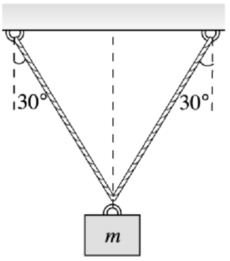
\includegraphics{\FileDepth/Activities/Suspended_Loudspeaker/Two_Cable_Speaker.pdf}
\end{figure}
}
\ProblemSub{\LoudHangB}{
(b) Draw a free-body diagram for the loudspeaker.
}
\Solution{\LoudHangBSol}{
\begin{figure}[h]
	\centering
	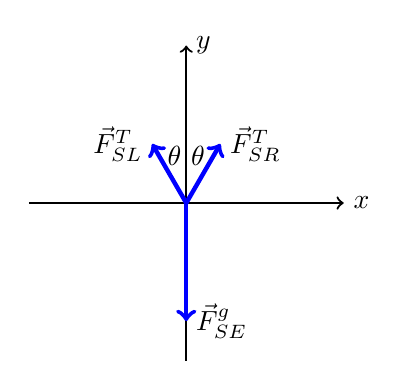
\begin{tikzpicture}
		\FBDaxes{0,0}{0}{axes}
		\FBDvectorMA{axes}{0.866}{60}{RT}
		\node[anchor=west] at (RTtip) {$\vec{F}^{T}_{SR}$};
		\node at (0.15,0.6) {$\theta$};
		\FBDvectorMA{axes}{0.866}{120}{LT}
		\node[anchor=east] at (LTtip) {$\vec{F}^{T}_{SL}$};
		\node at (-0.15,0.6) {$\theta$};
		\FBDvectorXY{axes}{0,-1.5}{FG}
		\node[anchor=west] at (FGtip) {$\vec{F}^{g}_{SE}$};
	\end{tikzpicture}
\end{figure}

Here, $\vec{F}^{T}_{SR}$ is the tension acting on the speaker from the cable on the right, and $\vec{F}^{T}_{SL}$ is the tension acting on the speaker from the cable on the left. Since there is only one object, I will drop the $S$ subscript in further calculations, and since there is only one force of gravity, I will drop both subscripts from it.
}
\ProblemSub{\LoudHangC}{
(c) Find the tension in each cable.
}
\Solution{\LoudHangCSol}{
First, we consider the $ x $-components. The loudspeaker is not accelerating, so
\[
F^{net}_{x} = ma_{x} = 0.
\]
The sum of the forces in this direction is
\[
F^{net}_{x} = F^{T}_{R}\sin\theta - F^{T}_{L}\sin\theta,
\]
therefore
\[
\begin{split}
	F^{T}_{L}\cancel{\sin\theta} & = F^{T}_{R}\cancel{\sin\theta} \\
	F^{T}_{L} & = F^{T}_{R}.
\end{split}
\]
This can be seen in the symmetry of the problem. Now, in the vertical direction, we have
\[
\begin{split}
	F^{net}_{y} & = ma_{y} = 0 \\
	F^{T}_{R}\cos\theta + F^{T}_{L}\cos\theta - F^{g} & = 0 \\
	2F^{T}_{R}\cos\theta - mg & = 0 \\
	F^{T}_{R} & = \frac{mg}{2\cos\theta} \\
	& = \frac{(25\text{ kg})(9.8\text{ m/s}^{2})}{2\cos(30^{\circ})} \\
	& \approx 140\text{ N}.
\end{split}
\]
Each cable has 140 N of tension in it.
}
\end{document}